\chapter{Projektformulering} \label{ch:Projektformulering}

\section*{Version}
\begin{table}[h]
	\centering
	\begin{tabularx}{\textwidth - 2cm}{|l|l| l|X|}
	\hline
	Dato	& Version	& Initialer & Ændring	\\ \hline
	26. februar & 1 & MHG & Første udkast. \\ \hline
	4. marts & 2 & LBS & Mindre rettelser efter første review. \\ \hline
	12. marts & 3 & MHG & Mindre rettelser efter fælles gennemlæsning. \\\hline
	16. maj & 4 & MHG & Mindre rettelser. \\\hline
	\end{tabularx}
\end{table}

\clearpage

\section{Beskrivelse}
Mange har prøvet at kaste sig ud i et nyt projekt, som for eksempel at dyrke frugt og grønt i drivhus, men pludselig glemmer man at vande, holde øje med temperaturen og lignende, og så er projektet gået i vasken.
 
AutoGreen hjælper den nye drivhusbruger med at holde styr på basale parametre som temperatur og fugtighed, men det er også for den mere erfarne drivhusbruger, som ønsker optimale forhold i drivhuset, eller som ønsker at vælge de mest egnede planter ud fra de forhold, der er i drivhuset.
 
Ved dyrkning af planter i et drivhus, er temperaturen en af de vanskeligste ting at kontrollere. Man er ikke altid hjemme, når drivhuset skal åbnes og lukkes, hvilket sjældent er samme tid på dagen; det afhænger af udendørstemperatur, skydække mm. 
Der findes mekaniske vinduesåbnere, som åbner og lukker et eller flere vinduer i drivhuset vha. en gasfyldt cylinder. 
Disse er dog forholdsvis upræcise, og reguleringen af temperaturen er langsom. Der er desuden ikke mulighed for at få ekstra varme tilført, hvilket kan være et stort problem, hvis vejret er ustabilt, særligt i starten af sæsonen. 
AutoGreen styrer temperaturen i drivhuset vha. en vinduesåbner, tovejs luftcirkulation og et varmelegeme. 
Dette giver en hurtig og præcis regulering af temperaturen. Varmelegemet tilfører ekstra varme, hvis der er for koldt i drivhuset. 
Dette kan meget vel redde planterne, hvis det viser sig, at man har plantet ud for tidligt, og det giver mulighed for at forspire i drivhuset, selv om drivhussæsonen ikke er startet. 
Hvis der er for varmt i drivhuset, åbner vinduet, og hvis dette ikke er tilstrækkeligt, anvendes også luftcirkulationen til at regulere temperaturen. 
Brugeren har mulighed for at vælge mellem forskellige måder at styre temperaturen på. Ønskes optimale forhold hurtigst muligt døgnet rundt, anvendes både varmelegeme, vinduesåbner og luftcirkulation. 
Brugeren kan også vælge fx at udelade brugen af varmelegemet eller luftcirkulationen, hvis en mere økonomisk temperaturregulering ønskes. 
 
En anden vigtig parameter for drivhusplanternes trivsel er selvfølgelig vanding, hvilket ligesom regulering af temperaturen kan være problematisk, hvis man ikke er hjemme, eller man ganske simpelt glemmer det. 
AutoGreen kan vha. en eller flere fugtmålere i drivhusjorden give brugeren besked om, at det er tid til at vande, ligesom et tilkoblet automatisk vandingssystem kan aktiveres. Et sådant vandingssystem er ikke en del af AutoGreen.
Forskellige planter kræver forskellig mængde vand, og brugeren har derfor mulighed for at bruge op til seks fugtmålere, som kan placeres i jorden ved forskellige plantetyper. 

AutoGreen måler desuden luftfugtighed og lysmængde i drivhuset; disse målinger logges sammen med målinger af fugtighed i jorden og temperaturmålinger. 
Brugeren kan vha. en database med de mest almindelige drivhusplanter vælge, hvad han vil dyrke i sit drivhus, eller han kan forsøge at optimere forholdene i drivhuset, hvis han ønsker bedre forhold for en bestemt type plante.  
Brugeren har mulighed for at tilføje ekstra planter i databasen. 

AutoGreen systemet kontrolleres af brugeren vha. en grafisk brugerflade med touch display, der realiseres på et Embest DevKit8000 Evaluation Board. \cite{lib:DK8000}
Alle sensorer og aktuatorer samt systemets masterenhed realiseres vha. PSoC4 udviklingsboards (CY8CKIT-042). \cite{lib:psoc4_guide}

\clearpage

\section{MoSCoW prioritering}
Ambitionen for dette projekt er som absolut minimum at realisere nedenstående punkter under \textit{"skal"}. 
Det forventes desuden at punkterne under \textit{"bør"} realiseres, men de har lavere prioritet.
Punkterne under \textit{"kan"} forventes ikke realiseret, og punkterne under \textit{"vil ikke..."} realiseres med sikkerhed ikke. 
Sidstnævnte punkter kan ses som udviklingsmuligheder i forhold til senere versioner af systemet. 

\begin{itemize}
	\item \textbf{Systemet skal:}
		\begin{itemize}
			\item Kunne monitorere temperaturen i drivhuset og regulere temperaturen i drivhuset vha. varmelegeme, åbning af vinduer og luftcirkulation.
			\item Give brugeren mulighed for at vælge varmelegeme og/eller luftcirkulation fra, hvis en mere økonomisk regulering af temperaturen ønskes. 
			\item Have et grafisk user interface.
		\end{itemize}
	\item \textbf{Systemet bør:}
		\begin{itemize}
			\item Måle jordfugtighed med op til seks sensorer i drivhuset og give brugeren besked på displayet om, at det er tid til at vande. 
			\item Måle Lysintensitet og luftfugtihed i drivhuset.
			\item Indeholde en log over alle målte parametre; jordfugtighed, temperatur, luftfugtighed og lysmængde. 
			Dataene præsenteres grafisk for brugeren.
			\item Indeholde en database over de mest almindelige drivhusplanter, så brugeren kan orientere sig om en plantes optimale forhold.
			\item Indeholde en systemlog, som noterer vigtige system hændelser.
		\end{itemize}
	\item \textbf{Systemet kan:}
		\begin{itemize}
			\item Sende besked til brugeren via email, om at det er tid til at vande.
			\item Tilkobles et automatisk vandingssystem, som aktiveres ved behov for vanding. 
			\item Give brugeren mulighed for at tilføje planter i databasen.
			\item Give brugeren mulighed for at kommunikere trådløst med systemet fra brugerfladen, så denne kan placeres fx inde i brugerens bolig. 
		\end{itemize}
	\item \textbf{Systemet vil ikke i denne version:}	
		\begin{itemize}
			\item Indeholde et kamera, og tilhørende billedarkiv, som giver brugeren mulighed for at følge planternes udvikling fra dag til dag. 
			\item Give brugeren mulighed for at agere med systemet via en app på dennes mobiltelefon. 
		\end{itemize}
\end{itemize}
\clearpage

\section{Rigt Billede}
\begin{figure}[h]
\centering 
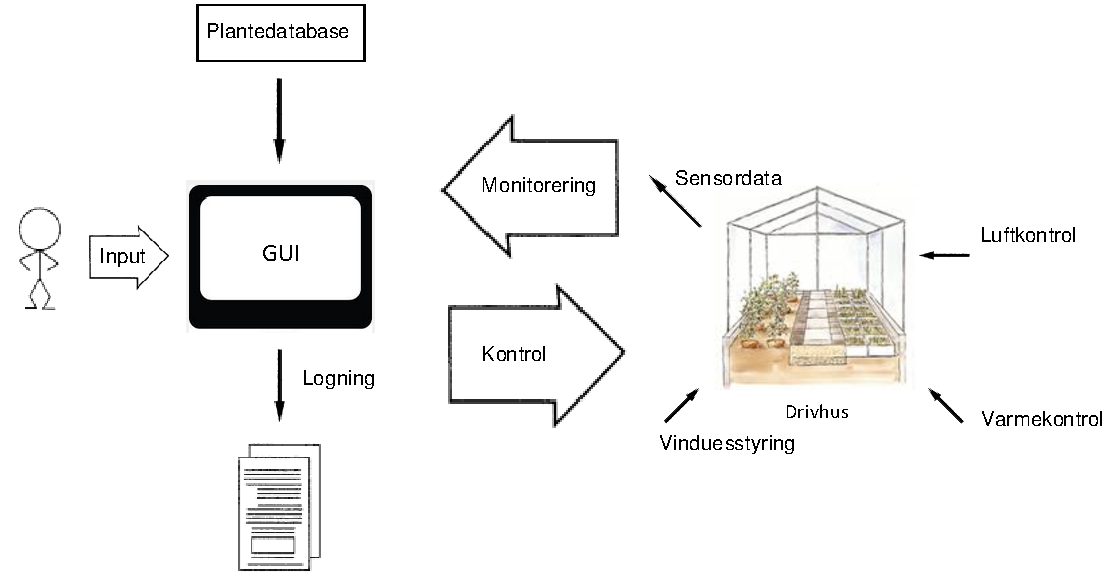
\includegraphics[width={\textwidth}] {../fig/Rigt_Billede.pdf}
\caption{AutoGreen Automatiseret Drivhus}
\label{fig:Rigt_Billede}
\end{figure}
